\section{Selecting curated Workflows}

%%%%%%%%%%%%%%%%%%%%%%%%%%%%%%%%%%%%%%%%%%%%%%%%%%%%%%%%%%%%%%%%%%%%%%%%%%%%%%%%
\begin{frame}
    \frametitle{Outline}
    \begin{columns}[t]
        \begin{column}{.5\textwidth}
            \tableofcontents[sections={1-9},currentsection]
        \end{column}
        \begin{column}{.5\textwidth}
            \tableofcontents[sections={10-18},currentsection]
        \end{column}
    \end{columns}
\end{frame}


%%%%%%%%%%%%%%%%%%%%%%%%%%%%%%%%%%%%%%%%%%%%%%%%%%%%%%%%%%%%%%%%%%%%%%%%%%%%%%%%
\begin{frame}
  \frametitle{What is this about?}
   \question[Questions]{\begin{itemize}
                         \item How do I get a workflow for a given scientific problem?
                         \item How do I run such an arbitrary workflow?
                        \end{itemize}
                       }
   \docs[Objectives]{\begin{enumerate}
                      \item Introducing the worfkflow catalogue?
                      \item Learning the difference between ``curation'' (what some people think) and ``curation'' (what really works)?
                     \end{enumerate}}
\end{frame}  

\subsection{The \texttt{Snakemake} Workflow Catalogue}

%%%%%%%%%%%%%%%%%%%%%%%%%%%%%%%%%%%%%%%%%%%%%%%%%%%%%%%%%%%%%%%%%%%%%%%%%%%%%%%%
\begin{frame}
 \frametitle{Selecting and Downloading from the Workflow Catalogue}
 You can find the \texttt{Snakemake} worfkflow catalogue, \lhref{https://snakemake.github.io/snakemake-workflow-catalog/?rules=true}{here}. It makes a difference between workflows which meet best-practice criteria - and those which do not.
 \begin{columns}
   \begin{column}{0.5\textwidth}
     You can download and run any workflow. \pause
     \warning{Except, you most likely cannot, because of a missing cluster configuration and some missing features.}
   \end{column}
   \begin{column}{0.5\textwidth}
     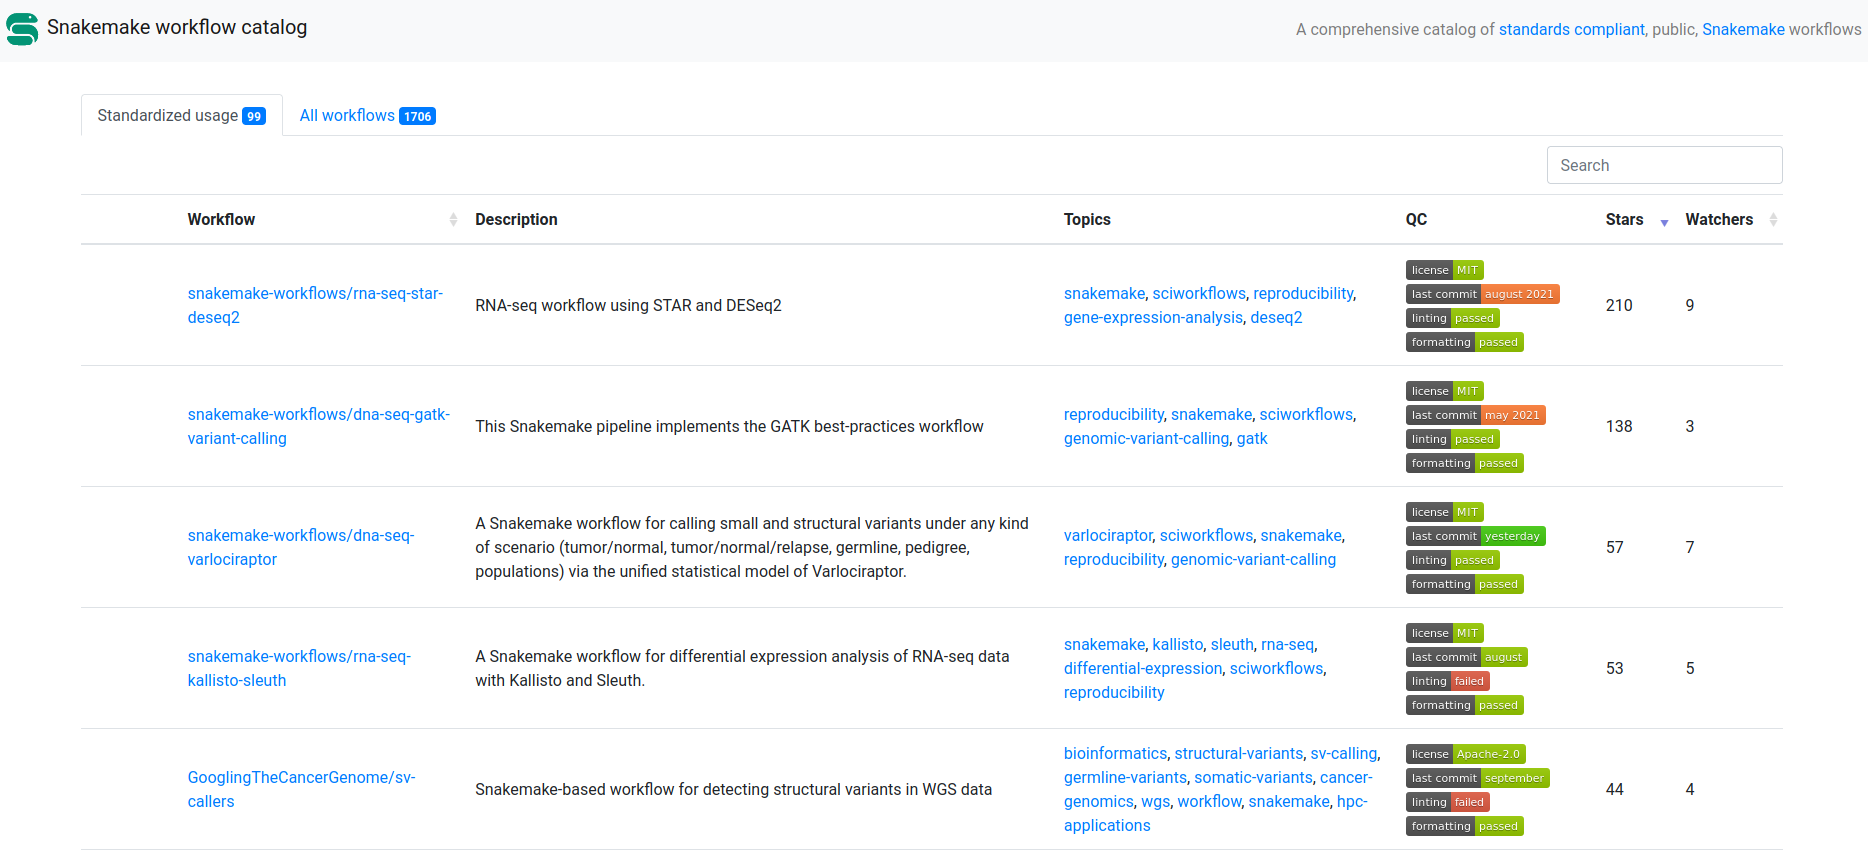
\includegraphics[width=\textwidth]{Snakemake/Snakemake_Workflow_Catalog.png}
   \end{column}
 \end{columns}

\end{frame}
